% The Bridge study — supplement (v3), FINAL typeset edition (2026-08-03).
% Source of truth: docs/research/BRIDGE-SUPPLEMENT.md (v3, prose-final).
% Companion to report.tex/report.pdf (Version 3). Unbounded length.
% Figure: figures/fig5_tooluse.pdf (regenerated on the repaired run rows by
% fig_f4_tooluse.py, census assertions inside the script).
% Build: latexmk -pdf supplement.tex
\documentclass[10pt]{article}

\usepackage[margin=1in]{geometry}
\usepackage[T1]{fontenc}
\usepackage[utf8]{inputenc}
\usepackage{lmodern}
\usepackage{microtype}
\usepackage{booktabs}
\usepackage{longtable}
\usepackage{graphicx}
\usepackage{amsmath,amssymb}
\usepackage{array}
\usepackage{enumitem}
\usepackage{xcolor}
\usepackage{titlesec}
\usepackage{caption}
\usepackage[hidelinks]{hyperref}
\urlstyle{tt}

\setlist{itemsep=1pt,topsep=2pt,parsep=0pt}
\setlength{\emergencystretch}{2.5em}
\tolerance=2000
\setlength{\textfloatsep}{8pt plus 2pt minus 3pt}
\setlength{\intextsep}{8pt plus 2pt minus 3pt}
\setlength{\abovecaptionskip}{5pt}
\titlespacing*{\section}{0pt}{1.8ex plus .6ex minus .3ex}{0.9ex plus .3ex}
\titlespacing*{\subsection}{0pt}{1.5ex plus .5ex minus .3ex}{0.7ex plus .2ex}
\titlespacing*{\paragraph}{0pt}{1.1ex plus .4ex minus .2ex}{0.8em}
\renewcommand{\arraystretch}{0.97}
\setlength{\LTpre}{5pt}
\setlength{\LTpost}{5pt}
\captionsetup{font=small,labelfont=bf}
\newcommand{\code}[1]{\texttt{#1}}
\newcommand{\best}[1]{\textbf{#1}}

% Supplement sections are S1..S14; use the section counter with an S prefix.
\renewcommand{\thesection}{S\arabic{section}}
\renewcommand{\thesubsection}{S\arabic{section}.\arabic{subsection}}

\title{\textbf{The Bridge Study --- Supplement (v3)}}
\author{Jack McCarthy\\
\normalsize WikiLean \,$\cdot$\, \url{https://wikilean.jackmccarthy.org}}
\date{Companion to the \textbf{Version 3} report --- August 2, 2026}

\begin{document}
\maketitle

\begin{center}
\begin{minipage}{0.92\textwidth}
\small
Companion to \code{docs/research/BRIDGE-REPORT.md} (version 3,
2026-08-02; typeset as \code{report.pdf}). Everything the main paper's
structure moved out lives here: the complete preregistration execution
inventory, raw-instrument tables and outage bases,
instrument-validation detail, exposure strata, sensitivity analyses,
the full tool-call census, the WF manual, review responses, the
changelog, and data availability. Section numbers \S Sn are cited from
the main paper. Nothing here is new evidence; every table is
recomputable from the file named beside it.
\end{minipage}
\end{center}

\section{Complete preregistration execution inventory}\label{s1}

Table~\ref{tab:inventory} lists every preregistered component, its
status, and the inferential consequence. Its sources are the
preregistration (\code{docs/research/BRIDGE-EXPERIMENT.md}, commit
\code{0d36f266}) and the claim-by-claim inventory in
\code{docs/research/review/verification-of-review-1.json} (prereg
section).

\begingroup\footnotesize
\begin{longtable}{@{}p{0.27\textwidth}p{0.10\textwidth}p{0.27\textwidth}p{0.27\textwidth}@{}}
\caption{Preregistration execution inventory.}
\label{tab:inventory}\\
\toprule
Preregistered component & Status & What actually happened & Inferential consequence \\
\midrule
\endfirsthead
\toprule
Preregistered component & Status & What actually happened & Inferential consequence \\
\midrule
\endhead
Five arms A--E, identical model/prompt/budget, tools-only difference & executed & 471 rows/arm (\code{bench/data/runs/}) & design intact \\
Per-tool call logging & executed & \code{tool\_calls\_by\_name} every row; full traces eval C/D/E + fresh (deviation 7) & enables trace attribution \\
Tier 1a ProofNet\# (371) & executed & 371/arm, scored & contaminated by construction (arm A 59.8\% on eval-341); paired deltas only \\
Tier 1b fresh set ($\sim$100) & executed & 100 tasks & holdout narrower than claimed (Brain indexes only; one later-fold leak) --- renamed post-Brain-index, 99/100 \\
Hallucinated-decl rate & executed & all tables & instrument required repair (\S S3); repaired rates are the report's \\
McNemar D-vs-E / D-vs-C + discordant tables & executed & main \S 4 & run on grounded typecheck, not the preregistered endpoint \\
10-min wall clock & executed & 600\,s timeouts & --- \\
Pre-campaign API requirements 1--8 & executed & implemented before campaign & --- \\
30-turn budget & \textbf{modified} & advisory only; overruns C 50/D 38/E 48 on the repaired rows (E 32 as-run --- outage rows masked overruns), max 88 & budget uncontrolled; \S S5 sensitivity \\
Determinacy pre-screen (exclude) & \textbf{modified} & post-hoc dual annotation (79\%, $\kappa\approx$0.20); 74-task subset, none excluded & subset analysis, not screened population \\
Arm-D production server & \textbf{modified} & production Worker code served locally over shipped shards & none material \\
Single-shot elaboration grading & \textbf{modified} & persistent REPL, same pins & none material \\
$\leq$4 typecheck calls in-loop & \textbf{modified} & no in-loop typechecking at all & halluc rate is a pure grounding measure \\
Skill/ToolSearch leak & \textbf{modified} & sealed before eval; 120 dev runs quarantined & dev split discarded, eval clean \\
Per-arm cost distributions & \textbf{modified} & means only (USD + wall-clock) & descriptive (\S S10) \\
faithful@budget (BEq+ equivalence) & \textbf{not executed} & grader a stub; zero judge files in campaign & primary endpoint missing; zero confirmatory results \\
LLM judge + 50-item human calibration & \textbf{not executed} (campaign) & harness existed unused; an \emph{uncalibrated} blind judge pass ran post-review (\S S11) & main \S 4.2 is exploratory only \\
tokens-to-solve (half the success criterion) & \textbf{not executed} & never computed (tokens recorded per row) & P2 untested as specified \\
3 reseeds + pass@k curves & \textbf{not executed} & one run per (task, arm) everywhere & no variance estimate anywhere \\
Second model class on primary set & \textbf{not executed} & Tier-1 all-Haiku; v2 all-Sonnet on different benchmarks & capability-band generality unknown \\
Preregistered success criterion & \textbf{not executed} & neither half graded as specified & zero confirmatory results \\
Tier 2 as specified (FATE-H + MPR-Prop proving, reflection loop) & \textbf{not executed} & replaced by exploratory v2: QR/MPR retrieval + one-shot SorryDB, arms N/F/W/U/WF & main \S\S 5--6 exploratory \\
PutnamBench & \textbf{not executed} & --- & --- \\
Tier 3a offline Erd\H{o}s set & \textbf{not executed} & --- & --- \\
Tier 3b live Erd\H{o}s queue & \textbf{not executed} & --- & --- \\
\bottomrule
\end{longtable}
\endgroup

\section{Tier-1: raw-instrument tables and analysis bases}\label{s2}

Sources for this section, all under \code{bench/analysis/}, are
\code{tier1\_reanalysis.\{py,json,md\}},
\code{part1\_fresh100\_v2.\{json,md\}},
\code{fresh\_clustered.\{py,json,md\}}, and
\code{success\_repaired.\{py,json,md\}}. Grading pins: eval-341 on Lean
v4.32.0-rc1 / Mathlib \code{a33a5ccd}; fresh-100 on Lean v4.33.0-rc1 /
Mathlib \code{9944fe29}; the checkout C/E's file tools read is
\code{61a5e4f338} (content $\sim$2026-07-10); ProofNet\# source pin
\code{PAug/ProofNetSharp @ a8da405f} (MIT).

\subsection{The three arm-E bases (raw instrument)}\label{s2:bases}

E's 31 infrastructure-dead rows (fresh\_069--099, contiguous
session-limit 429s; A--D verified zero errors) can be counted three
ways. Cells show grounded typecheck as n/N = \% [Wilson 95\% CI], on
the \textbf{raw oracle}:

\begin{center}\footnotesize
\begin{tabular}{@{}llll@{}}
\toprule
arm & errors-as-failures (n=100) & completed pairs (n=69) & post-repair (n=100) \\
\midrule
A & 20/100 = 20.0\% [13.3, 28.9] & 10/69 = 14.5\% [8.1, 24.7] & 20/100 = 20.0\% [13.3, 28.9] \\
B & 22/100 = 22.0\% [15.0, 31.1] & 12/69 = 17.4\% [10.2, 28.0] & 22/100 = 22.0\% [15.0, 31.1] \\
C & 25/100 = 25.0\% [17.5, 34.3] & 12/69 = 17.4\% [10.2, 28.0] & 25/100 = 25.0\% [17.5, 34.3] \\
D & 42/100 = 42.0\% [32.8, 51.8] & 28/69 = 40.6\% [29.8, 52.4] & 42/100 = 42.0\% [32.8, 51.8] \\
E & 16/100 = 16.0\% [10.1, 24.4] --- 31 infra errors & 16/69 = 23.2\% [14.8, 34.4] & 30/100 = 30.0\% [21.9, 39.6] \\
\bottomrule
\end{tabular}
\end{center}

Raw McNemar (exact binomial two-sided): errors-as-failures D-vs-E 32/6
p=2.4e-5 (conflates outage with behavior --- quarantined here);
completed-69 D-vs-E 18/6 p=0.023, D-vs-C 21/5 p=0.0025, D-vs-A 22/4
p=0.0005; post-repair full-100 D-vs-E 25/13 p=0.073, D-vs-C 28/11
p=0.0095, D-vs-A 29/7 p=0.0003, E-vs-A 19/9 p=0.087. Of the 31 repaired
E rows, 14 became successes.

\paragraph{Wald/McNemar mismatch note.} On the post-repair full-100 raw
table, the paired-Wald D$-$E risk-difference interval was
$[+0.0015, +0.2385]$ (barely excluding 0) while exact McNemar gave
p=0.073 --- a normal approximation over all 100 paired differences
versus a test conditioned on the 38 discordant pairs, landing on
opposite sides of $\alpha$=.05 near the boundary. This is why v3
replaces both with a single commit-clustered bootstrap whose interval
and p-value are read off the same resampling distribution.

\subsection{Raw vs repaired instrument, side by side}\label{s2:rawrep}

Repaired oracle = \code{halluc\_validation.py classify\_adjusted}
(rules R1--R5, \S S3), folded into success by
\code{success\_repaired.py}; success is monotone under the repair
(flags are only ever cleared). Affected rows (raw-flagged,
repaired-clean) and how many then typecheck:

\begin{center}\footnotesize
\begin{tabular}{@{}llll@{}}
\toprule
arm & affected (fresh) & typecheck pass & affected (eval-341) \\
\midrule
A & 17 & 1 & 39 \\
B & 18 & 0 & 45 \\
C & 38 & 8 & 68 \\
D & 17 & 6 & 47 \\
E & 39 & 7 & 81 \\
total & 129 & 22 & 280 \\
\bottomrule
\end{tabular}
\end{center}

\begin{center}\footnotesize
\begin{tabular}{@{}llll@{}}
\toprule
arm & raw k/n [Wilson 95] & repaired k/n [Wilson 95] & $\Delta$ \\
\midrule
A & 20/100 [13.3, 28.9] & 21/100 [14.2, 30.0] & +1 \\
B & 22/100 [15.0, 31.1] & 22/100 [15.0, 31.1] & +0 \\
C & 25/100 [17.5, 34.3] & 33/100 [24.6, 42.7] & +8 \\
D & 42/100 [32.8, 51.8] & 48/100 [38.5, 57.7] & +6 \\
E & 30/100 [21.9, 39.6] & 37/100 [28.2, 46.8] & +7 \\
\bottomrule
\end{tabular}
\end{center}

McNemar, both instruments:

\begin{center}\footnotesize
\begin{tabular}{@{}llllll@{}}
\toprule
pair & raw b/c & raw p & repaired b/c & repaired p & classification \\
\midrule
D vs E & 25/13 & 0.073 & 28/17 & 0.135 & ns $\to$ ns \\
D vs C & 28/11 & 0.0095 & 32/17 & 0.044 & sig $\to$ sig \\
D vs A & 29/7 & 0.00031 & 34/7 & 2.5e-5 & sig $\to$ sig \\
C vs A & 16/11 & 0.442 & 23/11 & 0.058 & ns $\to$ ns \\
E vs A & 19/9 & 0.087 & 24/8 & \best{0.007} & \best{ns $\to$ sig} \\
\bottomrule
\end{tabular}
\end{center}

Commit-clustered paired bootstrap (44 clusters, B=10,000; raw column
asserted byte-identical to \code{fresh\_clustered.json} before the
repaired column was computed):

\begin{center}\footnotesize
\begin{tabular}{@{}llll@{}}
\toprule
pair & raw RD [95\% CI] p & repaired RD [95\% CI] p & classification \\
\midrule
D $-$ E & $+0.120$ $[-0.049, +0.271]$ p=0.192 & $+0.110$ $[-0.089, +0.279]$ p=0.304 & ns $\to$ ns \\
D $-$ C & $+0.170$ $[+0.011, +0.314]$ p=0.040 & $+0.150$ $[-0.023, +0.302]$ p=0.100 & \best{sig $\to$ ns} \\
D $-$ A & $+0.220$ $[+0.093, +0.336]$ p=0.0014 & $+0.270$ $[+0.131, +0.395]$ p=0.0004 & sig $\to$ sig \\
\bottomrule
\end{tabular}
\end{center}

Note the two classification changes at $\alpha$=.05 cut in opposite
directions (E-vs-A strengthens, D-vs-C weakens) --- the repair is not a
thumb on either scale.

\subsection{Cluster census and sensitivity collapses}\label{s2:cluster}

The 100 tasks decompose into \textbf{44 distinct source commits},
\textbf{57 files}, and \textbf{59 name-stem families} (24
multi-member). The largest commit clusters are \code{87a6eccf} (9
tasks, the AntitoneOn sum--integral family), \code{49ed1b2d} (8,
bounded variation), \code{61303857} (5), two of size 4. On the raw
instrument, +7 of D's net +12 paired advantage over E comes from the
9-task commit (D 7/9, E 0/9) and +3 from the 8-task commit (D 4/8,
E 1/8) --- 83\% of the net effect in 2 of 44 commits.

All pairs $\times$ all clustering levels (raw instrument, paired
bootstrap RD [95\% CI] p):

\begin{center}
\resizebox{\textwidth}{!}{%
\begin{tabular}{@{}lllll@{}}
\toprule
pair & task-level (iid) & family-clustered & file-clustered & commit-clustered \\
\midrule
D $-$ E & $+0.120$ $[+0.000, +0.240]$ p=0.062 & $+0.120$ $[-0.044, +0.274]$ p=0.186 & $+0.120$ $[-0.044, +0.274]$ p=0.178 & $+0.120$ $[-0.049, +0.271]$ p=0.192 \\
D $-$ C & $+0.170$ $[+0.050, +0.290]$ p=0.0064 & $+0.170$ $[+0.021, +0.311]$ p=0.032 & $+0.170$ $[+0.021, +0.310]$ p=0.030 & $+0.170$ $[+0.011, +0.314]$ p=0.040 \\
D $-$ A & $+0.220$ $[+0.110, +0.330]$ p=0.0002 & $+0.220$ $[+0.080, +0.346]$ p=0.0028 & $+0.220$ $[+0.080, +0.344]$ p=0.0026 & $+0.220$ $[+0.093, +0.336]$ p=0.0014 \\
\bottomrule
\end{tabular}}
\end{center}

Family/file/commit-collapsed sensitivity (one unit per cluster,
majority and any-success rules) is tabulated in
\code{bench/analysis/fresh\_clustered.md} \S 4; under every collapse
D$-$E is a null (p $\geq$ 0.52), D$-$A survives the any-success
collapses (p=0.027--0.041), and the tie-free mean collapse gives D$-$E
$+0.043$ $[-0.104, +0.183]$ p=0.554, D$-$A $+0.157$ $[+0.043, +0.264]$
p=0.0064.

\subsection{Eval-341 (ProofNet\#) raw table and the repaired-instrument
gap}\label{s2:eval}

\begin{center}\footnotesize
\begin{tabular}{@{}lll@{}}
\toprule
arm & grounded typecheck (raw) & Wilson 95\% CI \\
\midrule
A & 204/341 = 59.8\% & [54.5, 64.9] \\
B & 198/341 = 58.1\% & [52.8, 63.2] \\
C & 218/341 = 63.9\% & [58.7, 68.9] \\
D & 219/341 = 64.2\% & [59.0, 69.1] \\
E & 208/341 = 61.0\% & [55.7, 66.0] \\
\bottomrule
\end{tabular}
\end{center}

The 280 raw-flagged repaired-clean eval rows (per-arm counts in S2.2)
exceeded the typecheck budget and were \textbf{not} re-typechecked; the
counts are hard upper bounds on per-arm gains, and the instrument-bias
direction (C/E over-flagged relative to D) applies to this table too.
Typecheck alone anti-correlates with grounding on this split (E led
typecheck at 83.3\% while trailing on hallucinations), reproducing
TheoremGraph's typecheck-is-not-a-signal finding at 15$\times$ their n.

\section{Hallucination-oracle validation detail}\label{s3}

Sources for this section are
\code{bench/analysis/halluc\_validation.\{py,json,md\}}, with blinded
intermediates in \code{bench/analysis/halluc\_blind/}.

\paragraph{Blinded protocol.} The audit drew a seeded (20260801),
stratified sample of 60 distinct cited names over arm $\times$
oracle-verdict strata (per arm: 6 flagged hallucinated, 5 exists, 1
renamed). The grader saw only the blinded sample (name + one context
line, shuffled, no verdicts) and raw \code{git grep} evidence at the
pinned trees (\code{61a5e4f338}, cross-checked at \code{9944fe2973}),
wrote truth labels, and only then unsealed the key. Grading required
namespace resolution, \code{to\_dual}-generation tracing,
\code{\_root\_.} declarations, and structure-field projections ---
exactly the care an exact-string oracle cannot apply.

\paragraph{Truth labels:} real 46 $\cdot$ nonexistent 4 $\cdot$
not\_a\_citation 9 (extractor noise) $\cdot$ renamed 1.

\paragraph{Confusion (oracle $\to$ truth):}

\begin{center}\footnotesize
\begin{tabular}{@{}llll@{}}
\toprule
 & truth real/renamed & truth nonexistent & truth not\_a\_citation \\
\midrule
oracle hallucinated (30) & 18 & 4 & 8 \\
oracle exists (25) & 24 & 0 & 1 \\
oracle renamed (5) & 5 & 0 & 0 \\
\bottomrule
\end{tabular}
\end{center}

\paragraph{Binary scores} (positive = hallucinated): strict precision
4/30 = \textbf{13.3\%} [5.3, 29.7], recall 4/4 = 100\% [51.0, 100];
lenient (noise rows excluded) precision 18.2\% [7.3, 38.5]. None of the
oracle's 30 negative verdicts (25 \emph{exists} + 5 \emph{renamed}) was
a missed fabrication (FN=0); read as verdicts rather than a pooled
negative class, 24/25 \emph{exists} names denoted real declarations
(one was extractor noise) and 4 of the 5 \emph{renamed} verdicts were
in truth real names.

\paragraph{The four confirmed fabrications} (zero-hit at both revs),
all from arms without formal tools: \code{FractionField} (A; real name
\code{FractionRing}), \code{Localization.At} (B;
\code{Localization.AtPrime}), \code{Ideal.vanishingLocus} (B;
\code{zeroLocus}/\code{vanishingIdeal}), \code{Nat.divisorSum} (B;
\code{ArithmeticFunction.sigma}).

\paragraph{The 26 false flags decompose into six mechanical modes:}
namespace short names standard under \code{open} (13), self-declared
theorem headers (4), dot-notation on a variable (5, e.g.\
\code{M.det}), comment prose (2), an import-line module name (1), a
mid-dot-chain fragment (1).

\paragraph{Repair rules R1--R5:} drop comment tokens, import-line
names, self-declarations, and single-letter dot-notation heads;
classify a name as existing if some single-segment prefix \code{NS.}
makes it an indexed declaration. Validation: the repaired classifier
agrees with the blinded truth on \textbf{59/60} (sole miss: the
mid-dot-chain fragment \code{Laurent.coeff.support}).

\paragraph{Run-level rates, both instruments} (n=100/arm;
citation-level shown for context --- citations cluster within runs, so
run-level carries the inference):

\begin{center}\scriptsize
\begin{tabular}{@{}lllllll@{}}
\toprule
arm & raw runs $\geq$1 halluc & raw citation-level & repaired runs $\geq$1 & repaired citation-level & R5 reclassified & R1--R4 dropped \\
\midrule
A & 54/100 [44.3, 63.4] & 94/443 = 21.2\% & 37/100 [28.2, 46.8] & 50/428 = 11.7\% & 29 & 15 \\
B & 48/100 [38.5, 57.7] & 76/429 = 17.7\% & 30/100 [21.9, 39.6] & 38/416 = 9.1\% & 25 & 13 \\
C & 49/100 [39.4, 58.7] & 108/517 = 20.9\% & 11/100 [6.3, 18.6] & 26/500 = 5.2\% & 65 & 17 \\
D & 23/100 [15.8, 32.2] & 32/472 = 6.8\% & 6/100 [2.8, 12.5] & 7/457 = 1.5\% & 10 & 15 \\
E & 49/100 [39.4, 58.7] & 107/505 = 21.2\% & 10/100 [5.5, 17.4] & 14/483 = 2.9\% & 71 & 22 \\
\bottomrule
\end{tabular}
\end{center}

Raw run-level McNemar: D-vs-E p=1.6e-4, D-vs-C p=6.9e-5 (run-level
ratio 2.13$\times$, not the citation-level 3.1$\times$). Repaired:
D-vs-E p=0.454, D-vs-C p=0.302, D-vs-A p=1.23e-7, D-vs-B p=3.9e-5,
E-vs-C p=1.0. Commit-clustered bootstrap versions of the significant
contrasts (\code{v3\_gate\_fixes.json}): D-vs-A $-0.310$
$[-0.446, -0.193]$ p=0.0002, E-vs-A $-0.270$ $[-0.396, -0.155]$
p=0.0002; the null D-vs-E / D-vs-C stay null (clustered p=0.44 /
0.31). The R5 column is the citation-style artifact quantified: C/E
write namespace-short names (65/71 reclassifications), D copies
fully-qualified names out of tool payloads (10).

\paragraph{Held-out revalidation of the repaired classifier (seed
20260802).} The five rules were formulated after the 60-name audit
unsealed, so 59/60 is an in-sample fit. A second blinded pass
(\code{bench/analysis/halluc\_holdout.\{py,json,md\}}; blinded
intermediates in \code{bench/analysis/holdout\_blind/}) sampled
\textbf{40 distinct cited names disjoint from the 60} (stratified per
arm: 4 raw-hallucinated, 3 raw-exists, 1 raw-renamed; shortfalls $\to$
exists) from the post-repair fresh rows, graded them blind under the
same evidence protocol (raw \code{git grep} at \code{61a5e4f338},
cross-check \code{9944fe2973}, run outputs for
self-declaration/variable resolution), and only then unsealed both
instruments' verdicts. Truth labels: real 31 $\cdot$ nonexistent 3
$\cdot$ not\_a\_citation 5 $\cdot$ renamed 1.

\begin{center}\footnotesize
\begin{tabular}{@{}lll@{}}
\toprule
metric (strict, n=40) & raw oracle & repaired classifier \\
\midrule
flagged-class precision & 3/20 = 15.0\% [5.2, 36.0] & 3/7 = 42.9\% [15.8, 75.0] \\
recall (true fabrications) & 3/3 = 100\% & 3/3 = 100\% \\
accuracy & 57.5\% & 90.0\% \\
binary agreement (the in-sample 59/60 measure) & 23/40 & \best{36/40 = 90.0\%} [76.9, 96.0] \\
\bottomrule
\end{tabular}
\end{center}

Sensitivity: reading the borderline \code{OrderedSemiring} (a class
removed by the ordered-algebra refactor; labeled renamed on the
Basis$\to$Module.Basis precedent) as nonexistent gives repaired
precision 4/7 = 57.1\%. The verdict: \textbf{directionally
replicates} --- the raw oracle's invalidity reproduces almost exactly
(13.3\%$\to$15.0\% precision), the repair transfers most of its value
(FPs on sampled flags 17$\to$4, accuracy 57.5\%$\to$90.0\%, zero FNs
for either instrument) --- but the in-sample fit was optimistic
(98.3\%$\to$90.0\% binary agreement, Fisher p=0.15), and a repaired
flag is roughly a coin toss, not a confirmation. The four residual FP
modes are ones R1--R5 never saw: multi-segment namespace short names
(\code{IsZero} $\leftarrow$ \code{CategoryTheory.Limits.IsZero}),
dot-notation on a namespaced def value
(\code{MeasureTheory.volume.restrict}), a multi-char local variable
(\code{M001}), and the removed-class borderline
(\code{OrderedSemiring}). Implications: the adjusted per-arm rates
likely overstate true hallucination by roughly 2$\times$ and should be
read as \textbf{upper bounds}; two of the four residual FP modes are
namespace-style-correlated (both held-out instances land in C/E-style
short-name arms), so the residual bias still runs \emph{against} the
free-text tool arms and cannot manufacture D's advantage; and all three
held-out confirmed fabrications (\code{Subgroup.torsion},
\code{Localization.map}, \code{Module.GeneralizedEigenspace}) sit in
the no-formal-tools arms A/B, as in-sample.

\section{Fresh-set exposure strata (full)}\label{s4}

The source is \code{bench/analysis/fresh\_exposure.\{py,json,md\}}
(original, snapshot basis), recomputed on the post-repair rows by
\code{bench/analysis/v3\_gate\_fixes.\{py,json\}} \S 1. Pinned tree
\code{61a5e4f338} (content $\sim$2026-07-10), the rev C/E's file tools
read. Outcomes below are the \textbf{post-repair rows} (E's 31 outage
rows replaced by their 2026-07-27 reruns) on the \textbf{raw}
instrument; the superseded snapshot-basis table (E's 429 rows counted
as failures) is preserved in \code{fresh\_exposure.md}.

Exposure counts (of 100): full dotted name in-tree verbatim
\textbf{37}; basename as a declaration header anywhere \textbf{64};
basename as header in the task's own module \textbf{51} (the stratum
basis); gold's commit an ancestor of the pin \textbf{49}. (Two tasks
are exposed despite post-pin merge commits --- measured on tree bytes,
not merge metadata.)

\begin{center}\footnotesize
\begin{tabular}{@{}lll@{}}
\toprule
arm & exposed (n=51) & unexposed (n=49) \\
\midrule
A & 9/51 = 17.6\% [9.6, 30.2] & 11/49 = 22.4\% [13.0, 35.9] \\
B & 8/51 = 15.7\% [8.2, 28.0] & 14/49 = 28.6\% [17.8, 42.4] \\
C & 11/51 = 21.6\% [12.5, 34.6] & 14/49 = 28.6\% [17.8, 42.4] \\
D & 24/51 = 47.1\% [34.1, 60.5] & 18/49 = 36.7\% [24.7, 50.7] \\
E & 15/51 = 29.4\% [18.7, 43.0] & 15/49 = 30.6\% [19.5, 44.5] \\
\bottomrule
\end{tabular}
\end{center}

McNemar by stratum, post-repair: D-vs-E exposed 14/5 p=0.064,
unexposed 11/8 p=0.648; D-vs-C exposed 18/5 p=0.0106, unexposed 10/6
p=0.454. The leak's direction favors C/E. \textbf{A correction to
earlier editions:} the snapshot-basis version of this table showed D's
edge over E strongest in the \emph{unexposed} stratum (17/3,
p=0.0026), and v2 concluded that D's advantage was ``strongest exactly
where there was nothing to leak.'' That pattern does not survive the E
repair --- 24 of E's 31 outage rows fell in the unexposed stratum, so
the stratum contrast was outage-driven. On the repaired rows D-over-E,
like D-over-C, is \emph{larger in the exposed stratum} (RD $+0.18$ vs
$+0.06$) and is a null unexposed; neither stratum is significant
alone. The merge-date split reproduces the repaired pattern
(before-pin 14/5 p=0.064; after-pin 11/8 p=0.648), and the
repaired-instrument sensitivity gives the same qualitative picture
(D-vs-E exposed 15/8 p=0.21; unexposed 13/9 p=0.52). The
judge-endpoint exposure split is \S S11.4.

\section{Turn-budget sensitivity}\label{s5}

The source is \code{tier1\_reanalysis.md} \S 5, corrected to the
post-repair rows by \code{v3\_gate\_fixes.py} \S 4. E overran the
advisory 30-turn budget on \textbf{48/100} repaired rows --- 16 of the
31 rerun rows plus 32 of the 69 originals; the earlier as-run count of
32 treated E's 31 outage rows (turns=1) as within budget, which also
inflated the old within-budget count (E 68) and the old n=45 pair
analysis. Corrected per-arm within-budget run counts: A 100, B 100,
C 50, D 62, E 52. Restricted to pairs where both arms stayed within
the advisory 30 turns (raw instrument, post-repair rows): D-vs-E n=35,
51.4\% vs 40.0\%, 7/3 discordant, p=0.34; D-vs-C n=35, 54.3\% vs
25.7\%, 11/1, p=0.0063; D-vs-A n=62, 46.8\% vs 25.8\%, 19/6,
p=0.0146. Consistent in direction; for D-vs-E, inconclusive within
budget.

\section{Tool-call census, cost/latency, and figure 5}\label{s6}

\paragraph{Tier-1 eval-split trace attribution}
(\code{bench/trace\_analysis.py}): 98--100\% of traced tool-arm runs
cite at least one declaration that surfaced in a tool result; 35\% of
arm-D eval runs cite a declaration from a
\code{brain\_bridge}/\code{brain\_transfer} result. Among
\emph{hallucinated} citations (raw oracle), the
checked-and-cited-anyway rate on eval rows is 35\% (C), 30\% (E), 13\%
(D); on the fresh split --- the paper's primary evidence base --- the
same statistic is C 44\%, D 34\%, E 61\%: verify-before-cite
discipline transferred imperfectly to the held-out set, and worst in
E.

\paragraph{v2 census} (figure: \code{figures/fig5\_tooluse.pdf} in the
typeset build, regenerated on the repaired run rows; the per-tool
counts quoted here are the as-run census --- the race repair raises
only F's means, since its 190 condemned rows had zero calls; basis
stated per clause): W averages 3.5 calls/run on QR-810 and 10.6 on
MPR, $\approx$4.0 pooled (QR-810 counts: decl\_exists 1,251 +
brain\_bridge 608 --- verify-then-cite made mechanical; pooled QR+MPR
counts: decl\_exists $\sim$1,473 + brain\_bridge $\sim$727); WF 4.6
pooled QR+MPR in a genuine dual-toolkit mix (decl\_grep $\sim$1.5k,
decl\_exists $\sim$0.9k, brain\_bridge $\sim$0.7k, decl\_read
$\sim$0.5k, loogle $\sim$0.4k); repaired F averages 2.8 (QR) and 8.2
(MPR) calls/run. Under the manual, \code{brain\_cell} misuse (63.3\%
failure over 482 W-arm calls) falls to a single call in WF.
Same-eval-set caveat as the manual (\S S8).

\begin{figure}[ht]
\centering
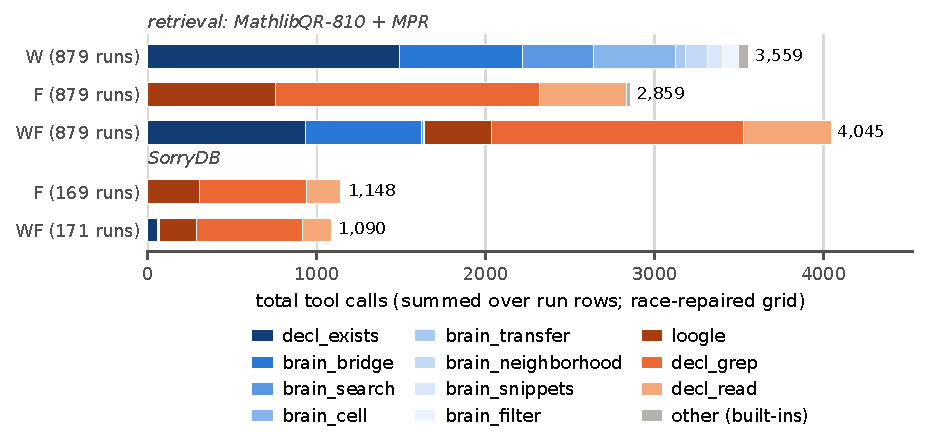
\includegraphics[width=0.92\textwidth]{figures/fig5_tooluse.pdf}
\caption{The v2 tool-use census by tool family (Brain blues, formal
oranges), summed over run rows --- regenerated on the race-repaired
grid (fig\_f4\_tooluse.py; census assertions against the \S S6 values
inside the script). The race repair raises only F's totals; the
prose census above quotes the as-run figures, basis stated per
clause.}
\label{fig:tooluse}
\end{figure}

\paragraph{The cold-start-race repair (grid provenance).} The \S 3.4
race was found by the U launch and repaired across seven commits.
\code{458891dc} built the U arm (bare W $\cup$ F union, no manual);
its first launch showed 13/49 rows with both MCP servers still
\code{pending} at the init event and zero tool calls, and
\code{834a130a} taught the runner to capture that init signature,
condemn-and-retry such rows, stagger the first wave, and raise the
attach timeout. \code{99a2075f} byte-archived the 194 affected grid
rows (F: 175 QR-810 + 15 MPR; W: 2 + 2; manifest of qids included) to
\code{bench/v2/runs/agent/race\_condemned\_archive/};
\code{f041928a} rerun all 194 attach-verified in place under the fixed
harness (the 4 stubborn W rows against the original fast-attaching
local worker --- the asymmetry that had spared W), leaving \textbf{zero
race rows in every arm $\times$ benchmark}; N/U/WF audit race-free
before and after (N has no MCP by design), and pre-existing
format/timeout failures (N 143+15, F 1, W 5, WF 1) are untouched.
\code{c1dea98f} landed the 879 attach-validated U rows (26 condemned
first attempts rerun; \$187.20); \code{322e84f5} and \code{dd3eb689}
are the union-ablation and repaired-grid analyses
(\code{union\_ablation.\{py,json,md\}},
\code{grid\_repaired.\{py,json,md\}}). Repair cost \$33.08. Scores
moved only for F (QR R@10 .8309$\to$.8457, nDCG .7901$\to$.8089; MPR
gR@10 .4532$\to$.5468); N/U/WF rows are byte-identical and W's
aggregates are unchanged at four decimals.

\paragraph{Per-query cost/latency (QR-810)} --- repaired grid,
recomputed from the final run rows (as-run table:
\code{retrieval\_repair.md} \S 3; CLI cost estimates under Max auth):

\begin{center}\footnotesize
\begin{tabular}{@{}llllll@{}}
\toprule
system & mean \$/query & mean wall s & median wall s & mean calls & mean turns \\
\midrule
N & 0.085 & 15.1 & 8.9 & 0.0 & 1.0 \\
F & 0.143 & 13.2 & 10.6 & 2.8 & 3.8 \\
W & 0.197 & 23.7 & 11.2 & 3.5 & 4.3 \\
U & 0.197 & 12.4 & 9.8 & 3.1 & 4.1 \\
WF & 0.207 & 15.2 & 12.5 & 4.2 & 5.2 \\
retriever-mode wikibrain & $\sim$0 & --- & --- & 1 & --- \\
\bottomrule
\end{tabular}
\end{center}

\paragraph{MPR (repaired grid):} N \$0.185/50.7\,s/0 calls $\cdot$ F
\$0.370/38.8\,s/8.2 $\cdot$ W \$0.459/62.6\,s/10.6 $\cdot$ U
\$0.403/33.1\,s/7.9 $\cdot$ WF \$0.418/38.2\,s/9.3. U-arm totals:
\$159.37 (QR-810) + \$27.84 (MPR) = \$187.20.

\paragraph{N format-repair detail} (\code{retrieval\_repair.md}):
symmetric tiered extraction (relaxed JSON $\to$ backticked names $\to$
bare dotted identifiers $\to$ compound tokens) over all assistant
text, identically for every arm's empty rows. QR: N 143 empty rows
$\to$ 104 repaired $\geq$1 name but only 12 recover the gold; strict
0.6333 $\to$ lenient 0.6481; oracle ceiling 0.8099. F/W/WF have 1/5/1
empty rows on the repaired grid (2/5/1 as-run) and move
$\leq$0.0012. The five W empties are 420\,s hard timeouts, not format
failures. MPR: N 15 empty $\to$ 1 gold recovered (0.2025 $\to$
0.2062). Per-tool provenance detail (surfaced-by-tool,
first-written-in, per-style tables):
\code{bench/analysis/retrieval\_provenance.md} --- an as-run trace
pass; its F row counts the 175 race rows' hits as memory (main \S 5
caveat).

\section{Snapshot rot: the detailed narrative}\label{s7}

The original SorryDB freeze (8 repositories, 164 tasks) was prepared
against sorrydb.org's SorryDB-2601 evaluation split with pinned
upstream commits. At verification time --- roughly six months after
the pins were minted --- 74 of 164 tasks (45\%) were unreproducible:
the pinned commits of GlimpseOfLean, LeanCourse25, and most Foundation
and SemicircleLaw tasks no longer exist on GitHub, their branches
force-pushed or rebased away. The rot is invisible to any cheap check:
GitHub's archive endpoint answers a preflight HEAD request for a dead
commit with HTTP 200, and only an actual fetch fails. The refreeze
(\code{bench/v2/sorrydb\_prep.py}, commit \code{db679e8d}) keeps
verified-fetchable pins only --- every task's repository archive
downloaded and its splice point confirmed --- yielding 171 tasks
across 10 repositories. Lesson for benchmark builders: a pin is not a
snapshot; archive the bytes, not the reference, and verify by
fetching, not by HEAD.

\section{The WF agent manual (verbatim) and its timeline}\label{s8}

\paragraph{Timeline (verified commit times).} N/F/W results committed
22:27 on 2026-07-24; the manual 00:30 on 2026-07-25; WF results 01:15
on 2026-07-25. The manual distills measurements from the same
evaluation queries WF was then scored on --- its bracketed figures
(per-style nDCG, the 63\% brain\_cell failure rate, the 143/810 format
failures, call counts) are the N/F/W/system-mode eval-set aggregates,
reproduced exactly. WF is therefore development evidence of a
maximally equipped, briefed agent, not an untouched test result. (v1
also misattributed the 63\% figure to ``the Tier-1 traces''; it is the
v2 W-arm figure --- 482 calls, 63.3\% failed.)

\begin{quote}\small
\code{bench/v2/AGENT\_MANUAL.md}, prepended verbatim to every WF-arm
prompt; a \textbf{post-hoc, benchmark-informed} artifact.
\end{quote}

\begingroup\footnotesize
\newcommand{\mhead}[1]{\par\medskip\noindent\textbf{#1}\par\smallskip}
\newcommand{\mtool}[1]{\par\smallskip\noindent\textit{#1}\par\nobreak}

\mhead{Tool manual: searching Mathlib with the Brain + formal search}

You have two complementary toolkits. Every claim in this manual is
measured from $\sim$5,500 logged tool calls across 3,500 benchmark runs
(Tier-1 + Bridge v2); numbers in brackets are those measurements.

\mhead{The mental model}

\begin{itemize}
\item \textbf{The Brain (wikibrain, 8 tools)} is a \emph{curated
  knowledge graph} joining informal mathematics (Wikipedia/Wikidata
  concepts, external databases) to Mathlib declarations. It knows what
  things \emph{mean} and how concepts relate --- but it only
  ``atomizes'' declarations that some concept, annotation, or tag
  claims ($\sim$12k of Mathlib's declarations). It is a map, not the
  territory.
\item \textbf{Formal search (3 tools)} operates on \emph{all} of
  Mathlib directly: type-pattern search (loogle), source grep, source
  reading. It knows everything that exists but nothing about what it
  means informally.
\end{itemize}

Rule of thumb: \textbf{route by what you're holding.} Holding a concept
described in words $\to$ start with the Brain. Holding a type shape or
name fragment $\to$ start with formal search. Always finish with
\code{decl\_exists} on every name you intend to output.

\mhead{Formal search tools}

\mtool{loogle}
Type-pattern and constant search (the public loogle.lean-lang.org
service).
\begin{itemize}
\item USE for: ``a lemma whose statement looks like
  \code{\_ * \_ $\leq$ \_ * \_}'', searches by involved constants
  (\code{Real.sqrt}, \code{tsum}), name substrings.
\item Strengths: covers ALL of Mathlib; $\sim$0\% call errors [578
  calls, 0 errors]; the best premise-finding tool --- the loogle+grep
  toolkit matched a specialist premise retriever [group-recall@10 0.453
  vs 0.461 SOTA].
\item Weaknesses: needs Lean syntax fluency; a wrong pattern silently
  returns unrelated hits; small result payloads mean you often need
  decl\_read next.
\end{itemize}

\mtool{decl\_grep}
Regex search over the Mathlib source checkout (ripgrep).
\begin{itemize}
\item USE for: name fragments (``cantor''), notation, docstring
  phrases, finding the file a declaration lives in.
\item Strengths: the workhorse [1,206 calls, 0\% errors]; catches
  things loogle's type index can't (comments, docstrings, naming
  conventions).
\item Weaknesses: lexical only --- if the concept's name doesn't appear
  in source, grep cannot find it (descriptive queries like ``special
  case of X'' score worst for grep-based agents [nDCG 0.384 vs the
  Brain's 0.523]).
\end{itemize}

\mtool{decl\_read}
Read declaration source (with surrounding context) from the checkout.
\begin{itemize}
\item USE for: verifying a candidate actually says what you think
  BEFORE citing it; getting exact signatures and hypotheses.
\item Strengths: ground truth for any decl in Mathlib [397 calls, 0\%
  errors].
\item Weaknesses: you need the file/name first --- it is a confirmation
  tool, not a discovery tool.
\end{itemize}

\mhead{Brain tools}

\mtool{brain\_bridge --- THE ENTRY POINT for informal$\to$formal}
Free text in, existence-verified declarations + owning atoms out, with
signatures, import lines, and one-hop dependency context.
\begin{itemize}
\item USE for: ``the concept described as $\langle$words$\rangle$'' ---
  especially nicknames and special-case descriptions, where the Brain's
  curated bonds beat grep [special\_case nDCG 0.523 vs 0.384; nickname
  0.779 vs 0.757].
\item CRITICAL LIMITATION (measured): its free-text matching is
  label/alias anchored, NOT semantic. A single call with a descriptive
  paraphrase usually misses [single-shot benchmark: 3.6\% R@10 vs 82\%
  for an agent that reformulates]. \textbf{Never accept one miss as the
  answer: reformulate 2--4 times} --- try the concept's canonical name,
  a synonym, the head noun alone. 8.9\% of calls return match:``none''
  [727 calls]; that response includes nearest-candidate suggestions ---
  read them.
\item The \code{hits} list is existence-verified; bond quality matters:
  \code{exact} means the decl IS the concept;
  \code{formalizes}/weaker bonds are nearby.
\end{itemize}

\mtool{brain\_search}
Fuzzy label + alias search returning atoms (cells).
\begin{itemize}
\item USE for: resolving a name you half-know into an atom id; browsing
  what the Brain calls something [400 calls, 0\% errors --- the
  reliable fallback when brain\_bridge misses].
\item Weaknesses: returns atoms, not ranked decls --- follow with
  brain\_cell on the winning atom.
\end{itemize}

\mtool{brain\_cell}
The full atom card: Lean code, Wikidata description, DB snippets,
organs.
\begin{itemize}
\item USE for: everything known about ONE object after bridge/search
  resolved it.
\item \textbf{THE \#1 MISUSE [63\% of 482 calls failed]: calling it
  with a bare \code{decl:Mathlib:Name} for an arbitrary declaration.}
  The Brain only has atoms for concept-joined decls; ``unresolvable
  key'' means \emph{no atom owns this decl}, NOT that the decl doesn't
  exist. For arbitrary decls use decl\_exists (works for all of
  Mathlib) and decl\_read for source. Call brain\_cell only with ids
  that came OUT of a Brain tool.
\end{itemize}

\mtool{decl\_exists --- THE DISCIPLINE TOOL}
Batch existence check for declaration names (backed by the full
oracle --- covers ALL of Mathlib, unlike brain\_cell).
\begin{itemize}
\item \textbf{USE ALWAYS, on every name you are about to output.} This
  is the measured difference between grounded and hallucinated
  citations: agents that verified before citing cut
  hallucinated-but-cited-anyway to 13\% vs 33\% for agents relying on
  fuzzy search results alone. It is cheap [1,473 calls, 0.1\% errors]
  and batched --- check 10 names in one call.
\item Also returns verified-rename suggestions for stale names.
\end{itemize}

\mtool{brain\_neighborhood}
The synapse graph around an atom (depends/links/relates, cursored).
\begin{itemize}
\item USE for: ``what connects to X'' --- finding the connecting lemma
  between two concepts, walking dependencies.
\item Weaknesses: needs a valid atom id [24.8\% of calls errored ---
  same unresolvable-key trap as brain\_cell; resolve the atom first].
\end{itemize}

\mtool{brain\_transfer / brain\_snippets / brain\_filter}
Narrower tools: label$\leftrightarrow$decl jumps for KNOWN labels
(transfer), stored source snippets (snippets), facet enumeration
(filter). High misuse rates when fed non-atom ids [40\%/57\% errors].
Prefer brain\_bridge/brain\_search entry; reach for these only on ids
the Brain already returned.

\mhead{Routing playbook}

\begin{center}\footnotesize
\begin{tabular}{@{}p{0.34\textwidth}p{0.58\textwidth}@{}}
\toprule
You are holding & Do this \\
\midrule
A concept in words & brain\_bridge $\to$ (miss?) reformulate $\to$ brain\_search $\to$ brain\_cell \\
A special case / nickname & brain\_bridge (the Brain's best terrain) \\
A type shape & loogle \\
A name fragment & decl\_grep \\
Premises for a proof & loogle + decl\_grep FIRST [0.453 vs 0.272], Brain for concept grounding \\
A candidate name to cite & decl\_exists (batch, always) $\to$ decl\_read if the statement matters \\
An atom id from any Brain tool & brain\_cell / brain\_neighborhood freely \\
A bare decl name needing info & decl\_exists + decl\_read --- NOT brain\_cell \\
\bottomrule
\end{tabular}
\end{center}

\mhead{Anti-patterns (each one measured in prior runs)}

\begin{enumerate}
\item \textbf{Citing unverified names.} 33\% of hallucinated citations
  came from agents that had search evidence in front of them and cited
  a wrong name anyway. decl\_exists is binary and kills this.
\item \textbf{One query, then giving up.} The single-call miss rate on
  descriptive queries is $\sim$96\%; agents that reformulate reach
  $\sim$82\%. Iteration IS the algorithm.
\item \textbf{brain\_cell as a generic decl inspector.} 63\% failure
  rate. Brain atoms $\neq$ all of Mathlib.
\item \textbf{Answering outside the requested format.} 143/810 no-tool
  runs were scored 0 for exactly this. Re-read the output contract
  before replying.
\item \textbf{Inventing tool names} (e.g.\ \code{logue},
  \code{lookie}). Use the names above.
\end{enumerate}
\endgroup

\medskip\noindent
\emph{(End of verbatim manual.)} Its bracketed measurements are the
as-run pre-repair aggregates as WF saw them --- e.g.\ the loogle+grep
premise figure it quotes as 0.453 is 0.547 on the repaired grid
(\S S6) --- and are preserved verbatim, not corrected.

\section{SorryDB: full bookkeeping}\label{s9}

The frozen split holds n=171 tasks/arm across 10 repositories, and all
203 candidate verdicts are definitive --- 183 kernel pass/fail plus 19
unspliceable and 1 verify-timeout that never reached the kernel
(commit \code{9682b3b1}; the 8 curve25519 stragglers verified as 0
proved). \code{verify.jsonl} carries 2 additional off-frozen N rows
verdicted \code{env\_broken} (205 lines total), correctly excluded
from the 203.

\begin{center}\footnotesize
\begin{tabular}{@{}llll@{}}
\toprule
 & N no tools & F formal & WF union+manual (post-hoc) \\
\midrule
run rows present & 168 & 169 & 171 \\
no output (timeout / no lean block) & 70 & 15 & 11 \\
honest give-up (literal \code{sorry}) & 40 & 83 & 86 \\
candidate proofs submitted & 58 & 71 & 74 \\
\textbf{proved (kernel)} & \best{2} & \best{9} & \best{10} \\
failed & 50 & 55 & 57 \\
unspliceable & 5 & 7 & 7 \\
verify timeout & 1 & 0 & 0 \\
proved / 171 & 1.2\% [0.3, 4.2] & 5.3\% [2.8, 9.7] & 5.8\% [3.2, 10.4] \\
repo-clustered boot 95\% CI & [0.0, 2.7] & [0.0, 10.7] & [0.0, 12.2] \\
proved / candidates & 3.4\% & 12.7\% & 13.5\% \\
total cost (USD) & 58.97 & 102.76 & 108.87 \\
cost per proved & 29.48 & 11.42 & 10.89 \\
mean wall-clock / task & 120\,s & 198\,s & 183\,s \\
\bottomrule
\end{tabular}
\end{center}

3 N and 2 F tasks lack run rows (runner losses). Distinct sorries
proved: 13; N's are a strict subset of F's and WF's; WF$\cap$F 6,
WF-only 4, F-only 3. Per-repo: PersistentDecomp N1/F3/WF3, LeanAPAP
0/4/5, MiscYD 1/2/2, the other seven repos 0 everywhere. WF$-$F:
$+0.0058$, repo-clustered 95\% CI $[+0.0000, +0.0185]$ (the lower
endpoint is exactly 0 because WF $\geq$ F in every repo; 34\% of
resamples show no difference or worse); task-level exact McNemar 4/3,
p=1.0. Cost-per-proved is bookkeeping only (unstable at 2/9/10
successes). The published SorryDB agentic best ($\sim$30\%) is not
comparable: different task subset, different protocol (published
agents iterate against the build; ours drafted one-shot).

\section{Per-arm cost tables}\label{s10}

\paragraph{Tier-1 campaign means per task} (all 471 runs/arm as run,
pre-repair; E's 31 error rows cost $\approx$0): A \$0.034 $\cdot$ B
\$0.048 $\cdot$ C \$0.140 $\cdot$ D \$0.121 $\cdot$ E \$0.128; mean
wall-clock C 116\,s, D 89\,s, E 106\,s. tokens-to-solve was never
computed, so P2 is untested; v1's ``cheaper and better'' framing
remains withdrawn. \textbf{Judge pass:} \$81.86 (CLI-reported) for 500
gradings + the 50-item re-grade. \textbf{v2 retrieval:} per-query
tables in \S S6. \textbf{SorryDB:} totals in \S S9.

\section{Blind LLM-judge grading: full tables}\label{s11}

Sources are \code{bench/analysis/judge\_fresh\_run.py} and
\code{judge\_fresh\_summary.\{py,json,md\}}, with the repaired-leg
conjunction from \code{bench/analysis/conjunction\_repaired.\{py,json\}}
(deterministic --- no sampling). Judge \code{claude-sonnet-5}; blind
(informal statement + gold with binders + candidate; no arm identity,
no tools, empty cwd); 500/500 rows, 0 errors; no-output rows
auto-fail. \textbf{Uncalibrated; exploratory.} The judge ran before
the oracle repair, so the conjunction is reported under both typecheck
instruments; the judge leg is identical in both.

\subsection{Fresh-100 rates}\label{s11:rates}

Strict equivalence (same proposition, same hypotheses):

\begin{center}\footnotesize
\begin{tabular}{@{}lll@{}}
\toprule
arm & k/n & Wilson 95\% CI \\
\midrule
A & 11/100 & [6.2, 18.6] \\
B & 9/100 & [4.8, 16.2] \\
C & 43/100 & [33.7, 52.8] \\
D & 8/100 & [4.1, 15.0] \\
E & 46/100 & [36.6, 55.7] \\
\bottomrule
\end{tabular}
\end{center}

Evaluated equivalence (mathematical equivalence, high confidence):
A 17/100 [10.9, 25.6] $\cdot$ B 16/100 [10.1, 24.4] $\cdot$ C 51/100
[41.3, 60.6] $\cdot$ D 19/100 [12.5, 27.8] $\cdot$ E 53/100
[43.3, 62.5].

Conjunction (grounded-typecheck $\wedge$ evaluated), both
instruments:

\begin{center}\footnotesize
\begin{tabular}{@{}lll@{}}
\toprule
arm & raw leg & repaired leg [Wilson 95] \\
\midrule
A & 8/100 & 8/100 [4.1, 15.0] \\
B & 9/100 & 9/100 [4.8, 16.2] \\
C & 16/100 & 20/100 [13.3, 28.9] \\
D & 15/100 & 16/100 [10.1, 24.4] \\
E & 18/100 & 21/100 [14.2, 30.0] \\
\bottomrule
\end{tabular}
\end{center}

Eight rows flip under the repair (C 4, E 3, D 1 --- the repaired-clean
typecheck passes that the judge also evaluated equivalent); B/A are
essentially untouched, and between-tool parity is preserved.

\subsection{McNemar, fresh-100}\label{s11:mcnemar}

Evaluated equivalence: D-vs-E 1/35 p=1.1e-9 $\cdot$ D-vs-C 3/35
p=6.7e-8 $\cdot$ D-vs-A 7/5 p=0.774 $\cdot$ E-vs-A 37/1 p=2.8e-10
$\cdot$ E-vs-B 39/2 p=7.8e-10 $\cdot$ E-vs-C 13/11 p=0.839.

Conjunction, raw leg: D-vs-E 6/9 p=0.607 $\cdot$ D-vs-C 8/9 p=1.0
$\cdot$ D-vs-A 9/2 p=0.065 $\cdot$ E-vs-A 11/1 p=0.0064 $\cdot$ E-vs-B
12/3 p=0.035 $\cdot$ E-vs-C 6/4 p=0.754.

Conjunction, repaired leg (\code{conjunction\_repaired.py}): D-vs-E
5/10 p=0.302 $\cdot$ D-vs-C 8/12 p=0.503 $\cdot$ D-vs-A 10/2 p=0.039
$\cdot$ E-vs-A 14/1 p=0.00098 $\cdot$ E-vs-B 14/2 p=0.0042 $\cdot$
E-vs-C 6/5 p=1.0. The only classification change at $\alpha$=.05 is
D-vs-A ns $\to$ sig --- a strengthening of tools-versus-none; every
between-tool conjunction contrast stays null under both instruments.

Commit-clustered bootstrap versions (44 clusters, B=10,000;
\code{v3\_gate\_fixes.json}): evaluated equivalence D-vs-E $-0.340$
$[-0.462, -0.220]$ p=0.0002, E-vs-A $+0.360$ $[+0.233, +0.469]$
p=0.0002; conjunction (repaired leg) D-vs-A $+0.080$
$[+0.011, +0.152]$ p=0.037, E-vs-A $+0.130$ $[+0.055, +0.226]$
p=0.0002, D-vs-E $-0.050$ $[-0.143, +0.021]$ p=0.247. No
classification changes: everything significant unclustered survives
clustering, and the nulls stay null.

\subsection{Completed-69 continuity}\label{s11:completed}

Evaluated: A 10/69 (.145) $\cdot$ B 9/69 (.130) $\cdot$ C 37/69 (.536)
$\cdot$ D 11/69 (.159) $\cdot$ E 37/69 (.536); D-vs-E 0/26 p=3.0e-8;
conjunction (raw leg): C 8/69 (.116) $\cdot$ D 10/69 (.145) $\cdot$
E 9/69 (.130), D-vs-E 4/3 p=1.0, D-vs-A 7/0 p=0.016; conjunction
(repaired leg): C, D, and E at exactly 11/69 (.159) each, D-vs-E 4/4
p=1.0, D-vs-A 8/0 p=0.0078.

\subsection{Exposure split (evaluated equivalence)}\label{s11:exposure}

\begin{center}\footnotesize
\begin{tabular}{@{}lll@{}}
\toprule
arm & exposed (n=51) & unexposed (n=49) \\
\midrule
A & 8/51 (.157) & 9/49 (.184) \\
B & 9/51 (.176) & 7/49 (.143) \\
C & 36/51 (.706) & 15/49 (.306) \\
D & 10/51 (.196) & 9/49 (.184) \\
E & 35/51 (.686) & 18/49 (.367) \\
\bottomrule
\end{tabular}
\end{center}

D-vs-E exposed: 1/26, p=4.2e-7. D-vs-E unexposed: 0/9, p=0.0039 ---
the inversion narrows off-leak but does not vanish; E produces more
judge-equivalent statements than D even where the gold was not
retrievable. The conjunction (S11.2) is where parity appears. This is
reported as measured; the human queue below is how it gets
adjudicated.

\subsection{Self-consistency and the human queue}\label{s11:queue}

Fixed 50-item seed-stratified re-grade (seed 20260727, 10/arm): strict
agreement 98.0\% (one flip), evaluated agreement 100.0\%. Human
grading queue = the 36 D/E-discordant tasks on evaluated equivalence
(they drive the D-vs-E McNemar): fresh\_002, 004, 006, 007, 011, 012,
013, 014, 019, 021, 023, 026, 027, 032, 044, 048, 049, 050, 051, 056,
057, 059, 062, 063, 064, 067, 069, 076, 077, 085, 086, 092, 094, 095,
096, 099.

\section{Responses to the external reviews}\label{s12}

Both reviews are preserved verbatim in \code{docs/research/review/}
(REVIEW-1.md, REVIEW-2.md), with our independent claim-by-claim
verification of review 1 in \code{verification-of-review-1.json}.

\subsection{Review 1 (of v1, 2026-07-27) --- actions taken in v2}
\label{s12:r1}

All eight concerns confirmed in substance (29 claims confirmed, 1
partial, 1 refuted). Two factual claims did not survive: MathlibMPR
does not cluster by PR (69 tasks, 69 distinct PRs), and arm E's 31
declaration-less runs were contiguous 429 errors, not interface
overload --- the second correction removed both the review's overload
reading and v1's error-inflated headline p=2.4e-5.

\begin{center}\footnotesize
\begin{tabular}{@{}p{0.04\textwidth}p{0.42\textwidth}p{0.46\textwidth}@{}}
\toprule
\# & Concern & Action \\
\midrule
1 & ``Success'' measures no semantic correctness & renamed grounded typecheck rate; judge pass; calibration owed \\
2 & D vs E does not isolate the join & ``join carries the effect'' retired; bundled-condition language; 2$\times$2 factorial on the roadmap \\
3 & Arm E failed its manipulation check & disclosed; yoked control on the roadmap \\
4 & Fresh set not isolated from formal-search sources & renamed post-Brain-index; exposure strata; frozen snapshots on the roadmap \\
5 & WF is test-set tuned & labeled post-hoc, benchmark-informed everywhere; provenance + timeline (\S S8); bare-union arm launched \\
6 & Independence and execution problems & declaration-clustered reanalysis; CIs throughout; disclosures \\
7 & Preregistered experiment incomplete; deviations silent & execution inventory (\S S1); register labels; zero-confirmatory up front \\
8 & SorryDB evidence thin & all 203 verdicts completed; WF-vs-F indistinguishable; cost claim deleted \\
\bottomrule
\end{tabular}
\end{center}

\subsection{Review 2 (of the v2 draft, 2026-08-01) --- actions taken in
v3}\label{s12:r2}

\begin{center}\footnotesize
\begin{tabular}{@{}p{0.05\textwidth}p{0.35\textwidth}p{0.52\textwidth}@{}}
\toprule
\# & Recommendation & Action in v3 \\
\midrule
1 & Lead with repaired full-100; one coherent paired inference & commit-clustered paired bootstrap is the only main-text framework; completed-69 and Wald/McNemar mismatch moved here (\S S2) \\
2 & Cluster the fresh set by commit/family & done (\code{fresh\_clustered.py}): 44 commits, 57 files, 59 families; all levels + collapses (\S S2.3); D$-$E widens exactly as predicted \\
3 & Human semantic evaluation & full 500-row blind judge complete with self-consistency; 36-task discordant queue defined; \textbf{human grading and calibration still pending} --- main \S 4.2 stays exploratory \\
4 & Factorial ablation & 2$\times$2 factorial not yet run; the bare-union U ablation is complete (main \S 5): the union is inert (U$-$F null everywhere), the WF gain is manual-driven on QR, and formal tools carry MPR; paper reframed around the bundled intervention and the tools-vs-none result per the review's conditional \\
5 & Characterize the Brain; retrieval provenance decomposition & done (\code{brain\_artifact.py}, main \S 3.1; \code{retrieval\_provenance.py}, main \S 5) \\
6 & Real related work (CRAMF, Aria, +) & done; every citation verified against arXiv on 2026-08-01 (\code{docs/research/review/related\_work\_notes.md}); comparison table in main \S 2 \\
7 & Correct two overclaims (memorization; ``clean verifier finding'') & memorization $\to$ benchmark-familiarity language (main \S 4.1); verifier finding restated after blinded oracle validation --- between-tool contrast dissolves under the repaired instrument (main \S 4.3), DDR cited as convergent evidence \\
8 & Repair the retrieval evaluation & symmetric lenient extraction for every arm, cost/calls columns, retriever-vs-agent blocks, Brain-gold coverage, provenance decomposition (main \S 5, \S S6); cold-start-race grid repair + U ablation complete; WF label kept \\
cuts & move manuals, inventories, strata, response tables, file maps out & this supplement is that move \\
\bottomrule
\end{tabular}
\end{center}

\section{Changelog}\label{s13}

\begin{itemize}
\item \textbf{v1 (2026-07-25).} Initial report. Headline claims later
  retired: ``the join carries the effect'' (p$<$0.0001 driven by an
  unrecognized outage), ``42\% success'' (no equivalence leg),
  ``contamination-proof fresh set'', WF as a SOTA row, cost-per-success
  claims.
\item \textbf{v2 (2026-07-31).} Post-review-1 corrected edition:
  metric renamed grounded typecheck; arm-E 429 block repaired; register
  labels (preregistered-modified / exploratory / corrective) and
  zero-confirmatory statement up front; exposure strata;
  declaration-clustered retrieval statistics; WF relabeled post-hoc;
  SorryDB verdicts completed; judge and union slots left open.
\item \textbf{v3 (2026-08-02, this edition).} Post-review-2
  restructure into an 8-page paper + this supplement. New evidence:
  blinded hallucination-oracle validation (13.3\% precision) + 5-rule
  repaired instrument, with all Tier-1 headline numbers recomputed
  under it; commit-clustered bootstrap as the single inferential
  framework; completed blind judge pass (500/500) with the three-layer
  contamination$\times$endpoint analysis; Brain artifact
  characterization; retrieval provenance decomposition (verification +
  routing, not content); N format-failure repair; the cold-start-race
  grid repair (194 rows rerun attach-verified; F QR R@10
  .831$\to$.846, MPR .453$\to$.547) with the bare-union U ablation and
  final contrast set; the repaired-leg judge conjunction; verified
  related work; cost columns; conflict/AI-use disclosures. Still open:
  human grading of the 36-task queue, judge calibration, the 2$\times$2
  factorial.
\item \textbf{v3 post-gate corrections (2026-08-03).} After an
  adversarial verification gate: held-out blinded revalidation of the
  repaired oracle (\S S3; flags become upper bounds); \S S4 exposure
  strata and \S S5 turn budgets recomputed on the post-repair rows
  (the ``strongest-where-nothing-to-leak'' claim retracted as
  outage-driven; E overruns 48/100); commit-clustered bootstraps
  extended to every significant \S 4.2/\S 4.3 contrast; Tier-1 attach
  audit; fresh-task provenance paragraph; five-arm judge Layer 1;
  census bases relabeled; assorted number and wording corrections
  (681, S6 fresh rates, SorryDB verdict categories, anchor
  provenance).
\end{itemize}

\section{Data availability and file map}\label{s14}

Everything needed to recompute the report lives in the private
preservation repository
\textbf{\code{Deicyde/wikilean-bridge-experiment}} (report at the
root; supplement under \code{report/}). Provenance commits below refer
to the WikiLean working repository.

\paragraph{Key commits.} \code{0d36f266} preregistration (2026-07-16)
$\cdot$ \code{f97e67e4} review-1 preservation + byte-preserved 429
archive $\cdot$ \code{19a90209} arm-E repair driver (MCP-attach
detection) $\cdot$ \code{64c48052} v2 corrective statistics
(tier1\_reanalysis, fresh\_exposure, retrieval\_clustered) $\cdot$
\code{9682b3b1} SorryDB kernel verdicts complete (203/203) $\cdot$
\code{36f3a472} report v2 + scored summary v2
(\code{bridge\_summary\_v2.json}) $\cdot$ \code{662db420} review-2
analyses (commit-clustered inference, blinded oracle validation, N
format repair, Brain artifact table, provenance decomposition) $\cdot$
\code{3cb8fa55} blind judge grading complete (500/500,
self-consistency, conjunction tables, human queue) $\cdot$
\code{9d10e44f} repaired-oracle Tier-1 recompute
(\code{success\_repaired}) $\cdot$ \code{458891dc} U-arm harness (bare
W $\cup$ F union, no manual) $\cdot$ \code{834a130a} cold-start-race
condemnation + staggered launches $\cdot$ \code{c1dea98f} U run rows
(879, attach-validated) $\cdot$ \code{322e84f5} union-ablation
analysis $\cdot$ \code{99a2075f} race-row archive (194 rows,
byte-preserved) $\cdot$ \code{f041928a} repaired F/W run rows (zero
race rows remain) $\cdot$ \code{dd3eb689} repaired-grid contrasts +
refreshed union ablation $\cdot$ \code{2a9f6b91} REPL routing fix
(``honest labels'').

\begin{center}\footnotesize
\begin{tabular}{@{}p{0.46\textwidth}p{0.46\textwidth}@{}}
\toprule
Path (preservation repo) & Contents \\
\midrule
\code{docs/research/BRIDGE-EXPERIMENT.md} & preregistration incl.\ deviations 1--7 \\
\code{docs/research/review/} & reviews 1--2 verbatim; verification-of-review-1.json; related\_work\_notes.md (verified citations) \\
\code{bench/*.py}, \code{bench/arms/} & Tier-1 harness: runner, scorer, REPL rig, trace analysis, arm manifests \\
\code{bench/data/bridge\_tasks.jsonl} & 371 ProofNet\# tasks (pinned fork, MIT) \\
\code{bench/data/fresh\_tasks.jsonl} & 100 post-Brain-index tasks + determinacy annotations + holdout check \\
\code{bench/data/runs/} & all 2,355 Tier-1 run rows incl.\ 31 repaired E rows \\
\code{bench/data/runs\_E\_fresh\_429\_archive/} & the 31 original 429 rows, byte-preserved \\
\code{bench/analysis/bridge\_summary\_v2.json} & scored fresh-500 summary + repair provenance \\
\code{bench/analysis/tier1\_reanalysis.*}, \code{fresh\_exposure.*}, \code{retrieval\_clustered.*} & v2 corrective statistics \\
\code{bench/analysis/fresh\_clustered.*}, \code{halluc\_validation.*} (+\code{halluc\_blind/}), \code{success\_repaired.*} & v3: clustered inference; blinded oracle validation; repaired-instrument recompute \\
\code{bench/analysis/halluc\_holdout.*} (+\code{holdout\_blind/}) & held-out blinded revalidation of the repaired oracle (40 disjoint names, seed 20260802) \\
\code{bench/analysis/v3\_gate\_fixes.\{py,json,md\}} & post-gate analyses: post-repair S4 strata, clustered \S 4.2/\S 4.3 bootstraps, Tier-1 attach audit, corrected turn budgets, five-arm judge table, fresh-task provenance \\
\code{bench/analysis/judge\_fresh\_run.py}, \code{judge\_fresh/}, \code{judge\_fresh\_summary.*} & blind judge pass (500 gradings + re-grade) \\
\code{bench/analysis/conjunction\_repaired.\{py,json\}} & judge conjunction under both typecheck instruments (deterministic) \\
\code{bench/analysis/retrieval\_repair.*}, \code{retrieval\_provenance.*}, \code{brain\_artifact.*} & v3: format repair; provenance decomposition (as-run trace pass); artifact characterization \\
\code{bench/analysis/union\_ablation.*}, \code{grid\_repaired.*} & U-arm bare-union ablation; race-repaired grid, before/after tables + final contrast set \\
\code{bench/v2/runs/agent/race\_condemned\_archive/} & the 194 original cold-start-race rows, byte-preserved with qid manifest \\
\code{bench/v2/} + \code{bench/v2/data/} + \code{bench/v2/runs/} & v2 harness, AGENT\_MANUAL.md, MathlibQR/MPR (CC BY 4.0), SorryDB freeze, all v2 run rows (repaired grid) with gzipped stream transcripts, verify.jsonl (203 verdicts) \\
\bottomrule
\end{tabular}
\end{center}

\paragraph{Recomputation entry points.} Tier-1 grading
\code{bench/score\_bridge.py}; repaired instrument
\code{bench/analysis/halluc\_validation.py} (\code{adjusted}) +
\code{success\_repaired.py} + held-out revalidation
\code{halluc\_holdout.py}; post-gate analyses
\code{v3\_gate\_fixes.py}; clustered inference
\code{fresh\_clustered.py}; exposure \code{fresh\_exposure.py}; judge
\code{judge\_fresh\_summary.py} + \code{conjunction\_repaired.py};
retrieval \code{bench/v2/score\_retrieval.py} +
\code{retrieval\_clustered.py} + \code{retrieval\_repair.py} +
\code{retrieval\_provenance.py}; repaired grid + union ablation
\code{grid\_repaired.py} + \code{union\_ablation.py}; artifact
\code{brain\_artifact.py}; SorryDB \code{bench/v2/verify\_sorrydb.py}.

\paragraph{External sources} (fetched and verified during the v2/v3
design sweeps): TheoremGraph arXiv:2606.25363 $\cdot$ LeanSearch
arXiv:2403.13310 $\cdot$ LeanSearch-v2 arXiv:2605.13137 +
github.com/frenzymath/LeanSearch-v2 $\cdot$ LeanExplore
arXiv:2506.11085 $\cdot$ SorryDB arXiv:2603.02668 + sorrydb.org
$\cdot$ FATE arXiv:2511.02872 $\cdot$ miniCTX arXiv:2408.03350 $\cdot$
LeanDojo arXiv:2306.15626 $\cdot$ LeanAgent arXiv:2410.06209 $\cdot$
Numina-Lean-Agent arXiv:2601.14027 $\cdot$ miniF2F-v2
arXiv:2511.03108 $\cdot$ ProofNet\#/ProofNetVerif arXiv:2406.07222
$\cdot$ benchmark-faults survey arXiv:2606.29493 $\cdot$ CRAMF
arXiv:2508.06931 $\cdot$ Aria arXiv:2510.04520 $\cdot$ DRIFT
arXiv:2510.10815 $\cdot$ DDR arXiv:2511.11990 (the last four verified
2026-08-01, \code{related\_work\_notes.md}).

\end{document}
